\subsection{Расчет профиля температур}

Для расчета профиля температур лопатки принимаем расход воздуха $G_в = 0.053 кг/c$, а величину зазора между дефлектором и
внутренней поверхностью лопатки $\delta = 1 мм$.

При расчете профиля температур лопатки при конвективно-пленочно охлаждении будем пользоваться следующей методикой:
\begin{enumerate}
	\item Зададим распределение приведенной скорости по корыту $\lambda_к \left( \overline{x} \right)$ и спинке $\lambda_с \left( \overline{x} \right)$:
		$$
			\lambda_к \left( \overline{x} \right) = 
			\left\{ 
				1 + 
				\left[ 
					\left( 
						\frac{\lambda_1}{\lambda_0}
					\right)^{0.5}
				\right]\overline{x}
			\right\}^{2} \lambda_0, \/\ \overline{x} = \frac{x}{l_к}
		$$
		$$
			\lambda_с \left( \overline{x} \right) = 
			\left\{ 
				1 + 
				\left[ 
					\left( 
						\frac{\lambda_1}{\lambda_0}
					\right)^{4}
				\right]\overline{x}
			\right\}^{0.25}\lambda_0, \/\ \overline{x} = \frac{x}{l_с}
		,$$
		где $l_к$ - длина профиля со стороны корыта, $l_с$ - длина профиля со стороны спинки, $\lambda_0$ - приведенная скорость на входе в лопаточный венец, $\lambda_1$ - приведенная скорость на выходе из лопаточного венца.

	\item Определим критическую скорость звука $a_{кр}$:
		$$
			a_{кр} = \sqrt{
				\frac{2k_г}{k_г + 1} R_г T_г^*
			}
		$$
	\item Определим скорость газа на корыте $v_к$ и на спинке $v_с$:
		$$
			v_к\left( x \right) = \lambda_к \left( \frac{x}{l_к} \right)
		$$
		$$
			v_c\left( x \right) = \lambda_к \left( \frac{x}{l_c} \right)
		$$
	Дальнейший расчет идентичен для спинки и корыта, поэтому скорость газа будем обозначать как $v_г$.
	\item Определим эквивалентную ширину щели:
		$$
			s = N_{отв} \frac{\pi d_{отв}^2}{4} \cdot \frac{1}{l},
		$$
		где $N_{отв}$ - количество отверстий, $d_{отв}$ - диаметр отверстия, $l$ - высота профильной части лопатки.
	\item Определим скорость газа в точке выдува воздуха:
		$$
			v_{г \/\ отв} = v_г\left( x_{отв} \right),
		$$
		где $x_{отв}$ - криволинейная координата отверстия.
	\item Определим статическую температуру газа в точке выдува воздуха:
		$$
			T_{г \/\ отв} = T_г^* - \frac{v_{г \/\ отв}}{2 c_{p \/\ г}}
		$$
	\item Определим статическое давление газа в точке выдува воздуха:
	 	$$
	 		p_{г \/\ отв} = \frac{p_г^*}{
	 			\left( 
	 				\frac{
	 					T_г^*
	 				}{
	 					T_{г \/\ отв}
	 				}
	 			\right)^\frac{k_г}{k_г - 1}
	 		}
	 	$$
	\item Определим статическую плотность газа в точке выдува воздуха:
	 	$$
	 		\rho_{г \/\ отв} = \frac{
	 			p_{г \/\ отв}
	 		}{
	 			R_г \cdot T_{г \/\ отв}
	 		}
	 	$$
	\item Определим скорость истечения воздуха из отверстия:
	 	$$
	 		v_{в \/\ отв} = \phi_{отв} \sqrt{
	 			\frac{2k_в}{k_в - 1}
	 		} R_в \theta \left( x_{отв} \right) 
	 		\left[ 
	 			1 - 
	 			\left( 
	 				\frac{
	 					p_{г \/\ отв}
	 				}{
	 					p_{в0}^*
	 				}
	 			\right)^\frac{k_в - 1}{k_в}
	 		\right],
	 	$$
	 	где $\phi_{отв}$ - коэффициент скорости, $\theta \left( x_{отв} \right)$ - температура воздуха в точке выдува, $p_{в0}^*$ - давление воздуха.
	\item Определим статическую плотность воздуха на выходе из отверстия:
		$$
			\rho_{в \/\ отв} = \frac{
				p_{г \/\ отв}
			}{
				R_в
				\left[
					\theta \left( x_{отв} \right) - \frac{v_{в \/\ отв}^2}{2c_{p \/\ в}}
				\right]
			}
		$$
	\item Определим плотность торможения воздуха на входе в отверстия:
		$$
			\rho_{в \/\ отв}^* = \frac{p_{в0}^*}{R_в \theta \left( x_{отв} \right) }
		$$
	\item Определим параметр вдува:
		$$
			m = \frac{\rho_{в \/\ отв} v_{в \/\ отв}}{\rho_{г \/\ отв} v_{г \/\ отв}}
		$$
	\item Определим число Рейнольдса по ширине щели:
		$$
			Re_s = \frac{
				\rho_{г \/\ отв} v_{г \/\ отв} s
			}{\mu_г\left( T_{г \/\ отв} \right)}
		$$
	\item Определим температурный фактор:
		$$
			\phi = \theta \left( x_{отв} \right) / T_г^*
		$$
	\item Определим эффективность пленки $\theta_{пл}\left( x \right)$:
		$$
			A\left( x \right) = Re_s^{-0.25} m^{-1.3} \phi^{-1.25}
			\left(
				\frac{
					x - x_{отв}
				}{
					s
				}
			\right)
		$$
		$$
			\theta_{пл}\left( x \right) = \left\{
				\begin{array}{@{}ll@{}}
					1.0, & \text{если}\ 0 < A \leq 3 \\
					\left( \frac{A}{3} \right)^{-0.285}, & \text{если} 3 \leq A < 11 \\
					\left( \frac{A}{7.43} \right)^{-0.95}, & \text{если} A \geq 11 \\
				\end{array}\right.
		$$
	\item Определим темперутуру пленки в случае нескольких рядов отверстий:
		$$
			T_{пл}^*\left( x \right) = T_г^* \cdot \prod_{i = 1}^{x_i \leq x}
				\left[
					\left(
						1 - \theta_{пл \/\ i}
					\right)
				\right] + 
				\sum_{i = 1}^{x_i \leq x} \left[
					\theta_{пл \/\ i}T_в^*\left( x_{отв \/\ j} \right)
					\prod_{j = i + 1}^{x_j \leq x} 
					\left(
						1 - \theta_{пл \/\ j}
					\right)
				\right]
		$$
	\item Определим коэффициент теплоотдачи пленки в случае нескольких рядов отверстий:
		$$
			\alpha_{пл}\left( x \right) = \alpha_{г}
			\prod_{i = 1}^{x_i \leq x} \left[
				1 + \frac{
					2m_i
				}{
					\frac{
						x - x_{отв \/\ i}
					}{s_i}
				}
			\right]
		$$
	\item По формуле истечения из сопла определим расход через ряд отверстий:
		$$
			G_отв = s \cdot l \cdot  \mu_{отв} \sqrt{
				\frac{2k_в}{k_в - 1} p_{в0}^*\rho_{в \/\ отв}^* 
				\left(
					\frac{
						p_{г \/\ отв}
					}{
						p_{в0}^*
					}
				\right)^\frac{2}{k_в}
				\left[
					1 - 
					\left(
						\frac{
							p_{г \/\ отв}
						}{
							p_{в0}^*
						}
					\right)^\frac{k_в - 1}{k_в}
				\right]
			}
		$$
	\item В общем случае зависимость расхода воздуха в зазоре от криволинейной координаты имеет вид:
		$$
			G_в \left( x \right) = G_{в0} - \sum_{i = 1}^{x_i \leq x} G_{отв \/\ i}
		$$

В данном расчете суммарный расход на охлаждение сопловых лопаток принимается равным
$G_0 = 45 \cdot 10^{-3} \/\ кг/c$ на лопатку, что при числе лопаток статора, равном 54, равно 4.89\% от суммарного расхода
воздуха.
В результате расчетов получим значения характерных параметров в отверстиях.

Значения характерных параметров в отверстиях корыта представлены в табл.~\ref{cool2:ps_hole_parameters}.
\begin{longtable}{|c|c|c|c|c|c|c|c|c|}
	\caption{Значения характерных параметров в отверстиях корыта}
	\label{cool2:ps_hole_parameters}
	\hline
	\textbf{№} &
	\textbf{$x, \/\ мм$} & 
	\textbf{$s, \/\ 10^{-3} \/\ мм$} &
	\textbf{$\phi_{отв}$} &
	\textbf{$\mu_{отв}$} &
	\textbf{$m$} & 
	\textbf{$\phi$} & 
	\textbf{$G_{отв}, \/\ 10^{-3} \/\ кг/с$} &
	\textbf{$G_{отв} / G_{в0}$} 
	\\ \hline
	\endhead
	<-<range .PSSolution.SlitsSolution>->
		<-<.Id>-> & 
		<-<.SlitInfo.Coord | MultiplyE3 | Round1>-> & 
		<-<.SlitInfo.Thickness | MultiplyE6 | Round1>-> &
		<-<.SlitInfo.VelocityCoef | Round2>-> &
		<-<.SlitInfo.MassRateCoef | Round2>-> &
		<-<.BlowingParameter | Round2>-> &
		<-<.TemperatureFactor | Round2>-> &
		<-<.MassRate | MultiplyE3 | Round2>-> &
		<-<.MassRateRel |Round3>-> 
		\\\hline
	<-<end>->	
\end{longtable}

Значения характерных параметров в отверстиях спинки представлены в табл.~\ref{cool2:ps_hole_parameters}.
\begin{longtable}{|c|c|c|c|c|c|c|c|c|}
	\caption{Значения характерных параметров в отверстиях спинки}
	\label{cool2:ss_hole_parameters}
	\hline
	\textbf{№} &
	\textbf{$x, \/\ мм$} & 
	\textbf{$s, \/\ 10^{-3} \/\ мм$} &
	\textbf{$\phi_{отв}$} &
	\textbf{$\mu_{отв}$} &
	\textbf{$m$} & 
	\textbf{$\phi$} & 
	\textbf{$G_{отв}, \/\ 10^{-3} \/\ кг/с$} &
	\textbf{$G_{отв} / G_{в0}$} 
	\\ \hline
	\endhead
	<-<range .SSSolution.SlitsSolution>->
		<-<.Id>-> & 
		<-<.SlitInfo.Coord | MultiplyE3 | Round1>-> & 
		<-<.SlitInfo.Thickness | MultiplyE6 | Round1>-> &
		<-<.SlitInfo.VelocityCoef | Round2>-> &
		<-<.SlitInfo.MassRateCoef | Round2>-> &
		<-<.BlowingParameter | Round2>-> &
		<-<.TemperatureFactor | Round2>-> &
		<-<.MassRate | MultiplyE3 | Round2>-> &
		<-<.MassRateRel |Round3>-> 
		\\\hline
	<-<end>->	
\end{longtable}


	\item Определим коэффициент теплоотдачи от газа на входной кромке лопатки $\alpha_{г.вх.кр.}$:
		$$
			\alpha_{г.вх.кр.} = 0.74 \frac{
				\lambda_г
			}{
				d_{вх.кр.}
			}\sqrt{
				\frac{
					\rho_г \cdot c_a \cdot d_{вх.кр.}
				}{
					\mu_г
				}
			} =
		$$
		$$
			= 0.74 \frac{
				<-<.Gas.LambdaGas | MultiplyE3 | Round1>-> \cdot 10^{-3}
			}{
				<-<.Geom.DInlet | MultiplyE3 | Round2>-> \cdot 10^{-3}
			}\sqrt{
				\frac{
					<-<.Gas.RhoGas | Round1>-> \cdot 
					<-<.Gas.Ca | Round1>-> \cdot 
					<-<.Geom.DInlet | MultiplyE3 | Round2>-> \cdot 10^{-3}
				}{
					<-<.Gas.MuGas | MultiplyE6 | Round1>-> \cdot 10^{-6}
				}
			} = <-<.Gas.AlphaGasInlet | Round1>-> \/\ Вт/\left( м^2 \cdot К\right)
		$$
	\item Определим коэффициент теплоотдачи на спинке на расстоянии $\frac{1}{3} b_a$ $\alpha_{г.вых.кр.}$:
		$$
			\alpha_{г.вых.кр.} = 1.5 \alpha_г = 
			1.5 \cdot <-<.Gas.AlphaMean | Round1>-> = <-<.Gas.AlphaGasOutlet | Round1>-> Вт/\left( м^2 \cdot К\right)
		$$
	\item Определим коэффициент теплоотдачи на остальной выпуклой части (спинке) $\alpha_{г.сп.}$:
		$$
			\alpha_{г.сп.} = 0.6 \alpha_г = 0.6 \cdot <-<.Gas.AlphaMean | Round1>-> = <-<.Gas.AlphaGasSS | Round1>-> Вт/\left( м^2 \cdot К\right)
		$$
	\item Определим коэффициет теплоотдачи на вогнутой части профиля (корыте) $\alpha_{г.кор.}$:
		$$
			\alpha_{г.кор.} = \alpha_г = <-<.Gas.AlphaMean | Round1>-> = <-<.Gas.AlphaGasPS | Round1>-> Вт/\left( м^2 \cdot К\right)
		$$
	\item Коэффициент теплоотдачи от стенки к охлаждающему воздуху зависит от его температуры и определяется следующим уравнением $\alpha_{в}$:
		$$
			\alpha_{в} = 0.02 \cdot \frac{
				\lambda_{в}
			}{
				2\delta
			} \left( 
				\frac{
					G_в
				}{
					l
				} \cdot \frac{
					1
				}{
					\mu_{в}
				}
			\right)^{0.8}
		$$

	\item Уравнение теплообмена между охлаждающим воздухом и газом имеет вид:
		$$
			\frac{d\theta}{dx} = \frac{
				2
			}{
				G_в C_{p \/\ в}
			} \frac{
				k_x
			}{
				\alpha_г
			} \left( 
				T_{пл}^* - \theta
			\right),
		$$
	где $k_x$ - коэффициент теплопередачи, определяемый уравнением
		$$
			k_x = \frac{1}{
				\frac{1}{
					\alpha_{пл}
				} + 
				\frac{1}{
					\alpha_в
				} + 
				\frac{\Delta}{\lambda_м}
			}
		$$
	\item Уравнение теплового баланса малого элемента стенки лопатки
	$$
		\frac{d^2T_{ст}}{d x^2} = \frac{1}{\lambda \delta}
		\left[
		\left(
		\alpha_{пл} + \alpha_в
		\right) \theta -
		\left(
		\alpha_{пл} T_{пл} + \alpha_в T_в
		\right)
		\right],
	$$
	где $T_{ст}$, К - температура материала лопатки,
	$\lambda$ Вт/м - теплопроводность материала лопатки,
	$\delta$, м - толщина стенки,
	$\alpha_{пл}$, $Вт/м^2$ - коэффициент теплоотдачи пленки пленки газа снаружи лопатки,
	$\alpha_в$, T_{ст} - коэффициент теплоотдачи воздуха внутри лопатки,
	$T_{пл}$, К - температура пленки,
	$T_в$, К - температура охлаждаюущего воздуха.

	Численно решая уравнение теплообмена, получим распределение параметров по спинке и корыту.
	Распределение параметров газа по спинке представлено в табл.~\ref{cool2:ss_gas_parameters}.
		\begin{longtable}{|c|c|c|c|c|c|}
		\caption{Распределение параметров газа по спинке}
		\label{cool2:ss_gas_parameters}
		\hline
		\textbf{№} &
		\textbf{$x, \/\ м$} & 
		\textbf{$\alpha_{пл} \/\ Вт/\left(м^2 \cdot К\right)$} & 
		\textbf{$\alpha_в \/\ Вт/\left(м^2 \cdot К\right)$} & 
		\textbf{$\theta_x, \/\ К$} & 
		\textbf{$T_{ст.x}, \/\ К$} 
		\\ \hline
		\endhead
		<-<range .Gas.SSRows>->
			<-<.Id>-> & 
			<-<.X | MultiplyE3 | Round3>-> & 
			<-<.AlphaGas | Round1>-> & 
			<-<.AlphaAir | Round1>-> &
			<-<.TAir | Round1>-> & 
			<-<.TWall | Round1>->
			\\\hline
		<-<end>->
		\end{longtable}

	Распределение параметров газа по корыту представлено в табл.~\ref{cool2:ps_gas_parameters}.
		\begin{longtable}{|c|c|c|c|c|c|}
		\caption{Распределение параметров газа по корыту}
		\label{cool2:ps_gas_parameters}
		\hline
		\textbf{№} &
		\textbf{$x, \/\ 10^{-3} м$} & 
		\textbf{$\alpha_{пл} \/\ Вт/\left(м^2 \cdot К\right)$} & 
		\textbf{$\alpha_в \/\ Вт/\left(м^2 \cdot К\right)$} & 
		\textbf{$\theta_x, \/\ К$} & 
		\textbf{$T_{ст.x}, \/\ К$} 
		\\ \hline
		\endhead
		<-<range .Gas.PSRows>->
			<-<.Id>-> & 
			<-<.X | MultiplyE3 | Round3>-> & 
			<-<.AlphaGas | Round1>-> & 
			<-<.AlphaAir | Round1>-> &
			<-<.TAir | Round1>-> & 
			<-<.TWall | Round1>->  
			\\\hline
		<-<end>->	
		\end{longtable}

\end{enumerate}

Распределение температуры газа, воздуха и металла по профилю лопатки при исходном варианте установки
(без дожимающего компрессора) показано на рис.~\ref{img:cool_gas_parameters_no_front}.
\begin{figure}[H]
    \centering
	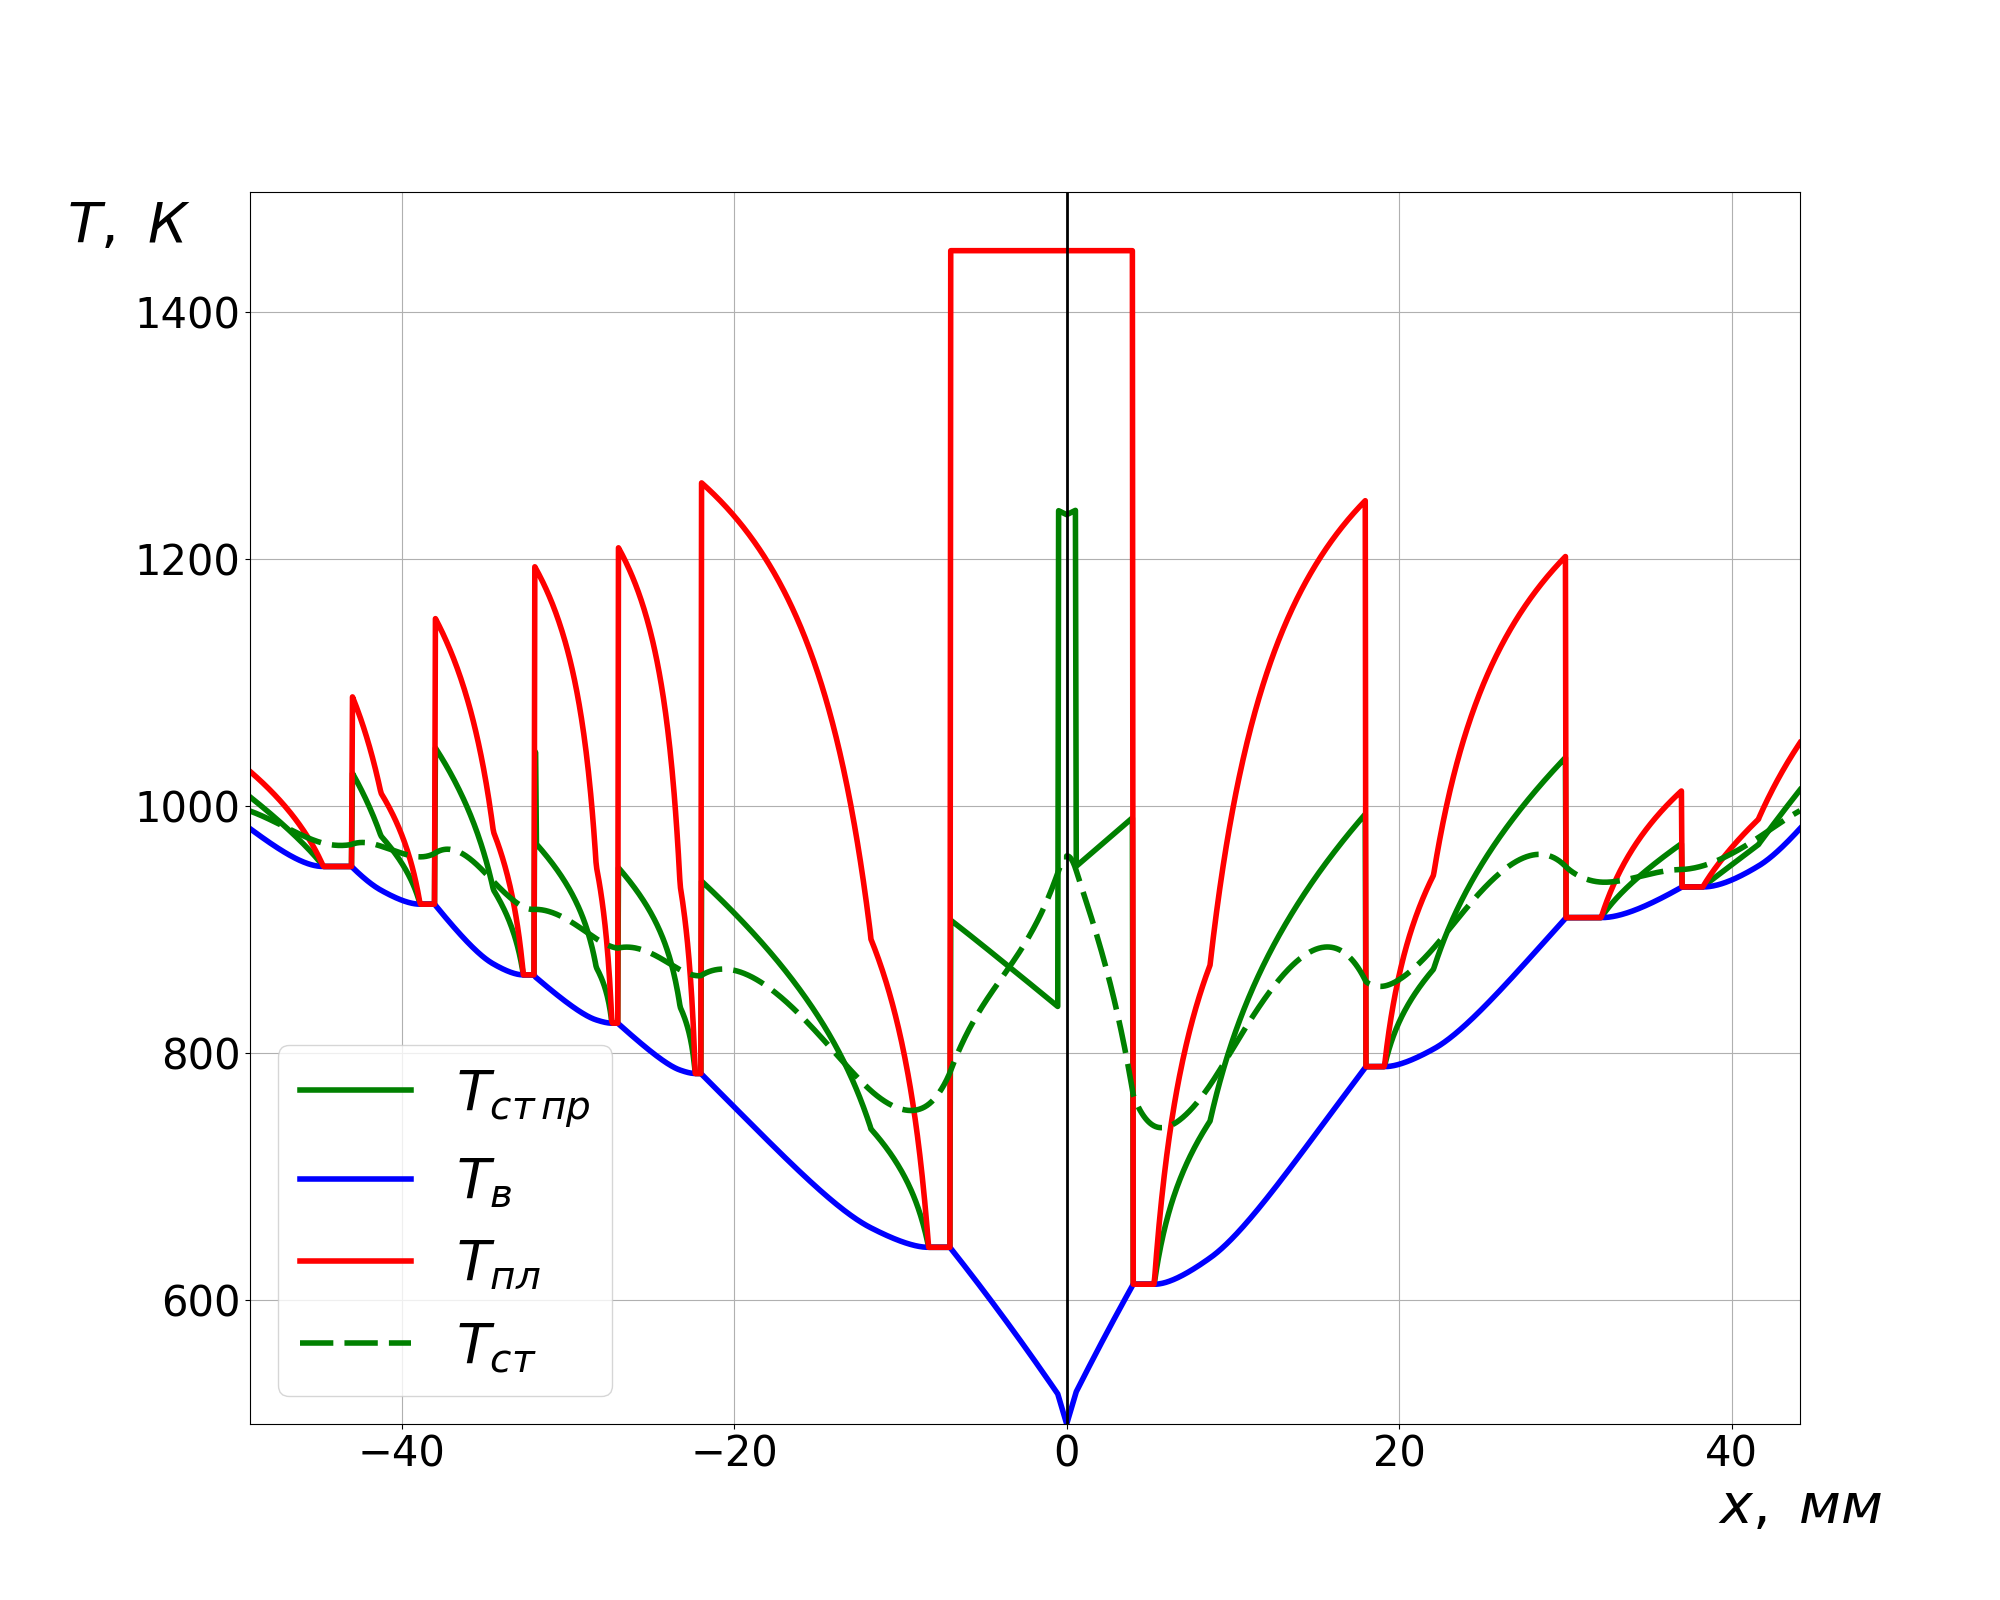
\includegraphics[scale=0.3]{cooling_2_t_no_front}
	\caption{Распределение температур газа, воздуха и металла, $T_{ст \ пр}$ - температура материала лопатки, полученная
	по приближенном методике, $T_в$ - температура охлаждающего воздуха, $T_{пл}$ - температура пленки, $T_{ст}$ -
	температура материала лопатки, полученная по уточненной методике}
	\label{img:cool_gas_parameters_no_front}
\end{figure}

Вариант с выдувом в лобовой точке (с дожимающим компрессором) показан на рис.~\ref{img:cool_gas_parameters_front}.
\begin{figure}[H]
    \centering
	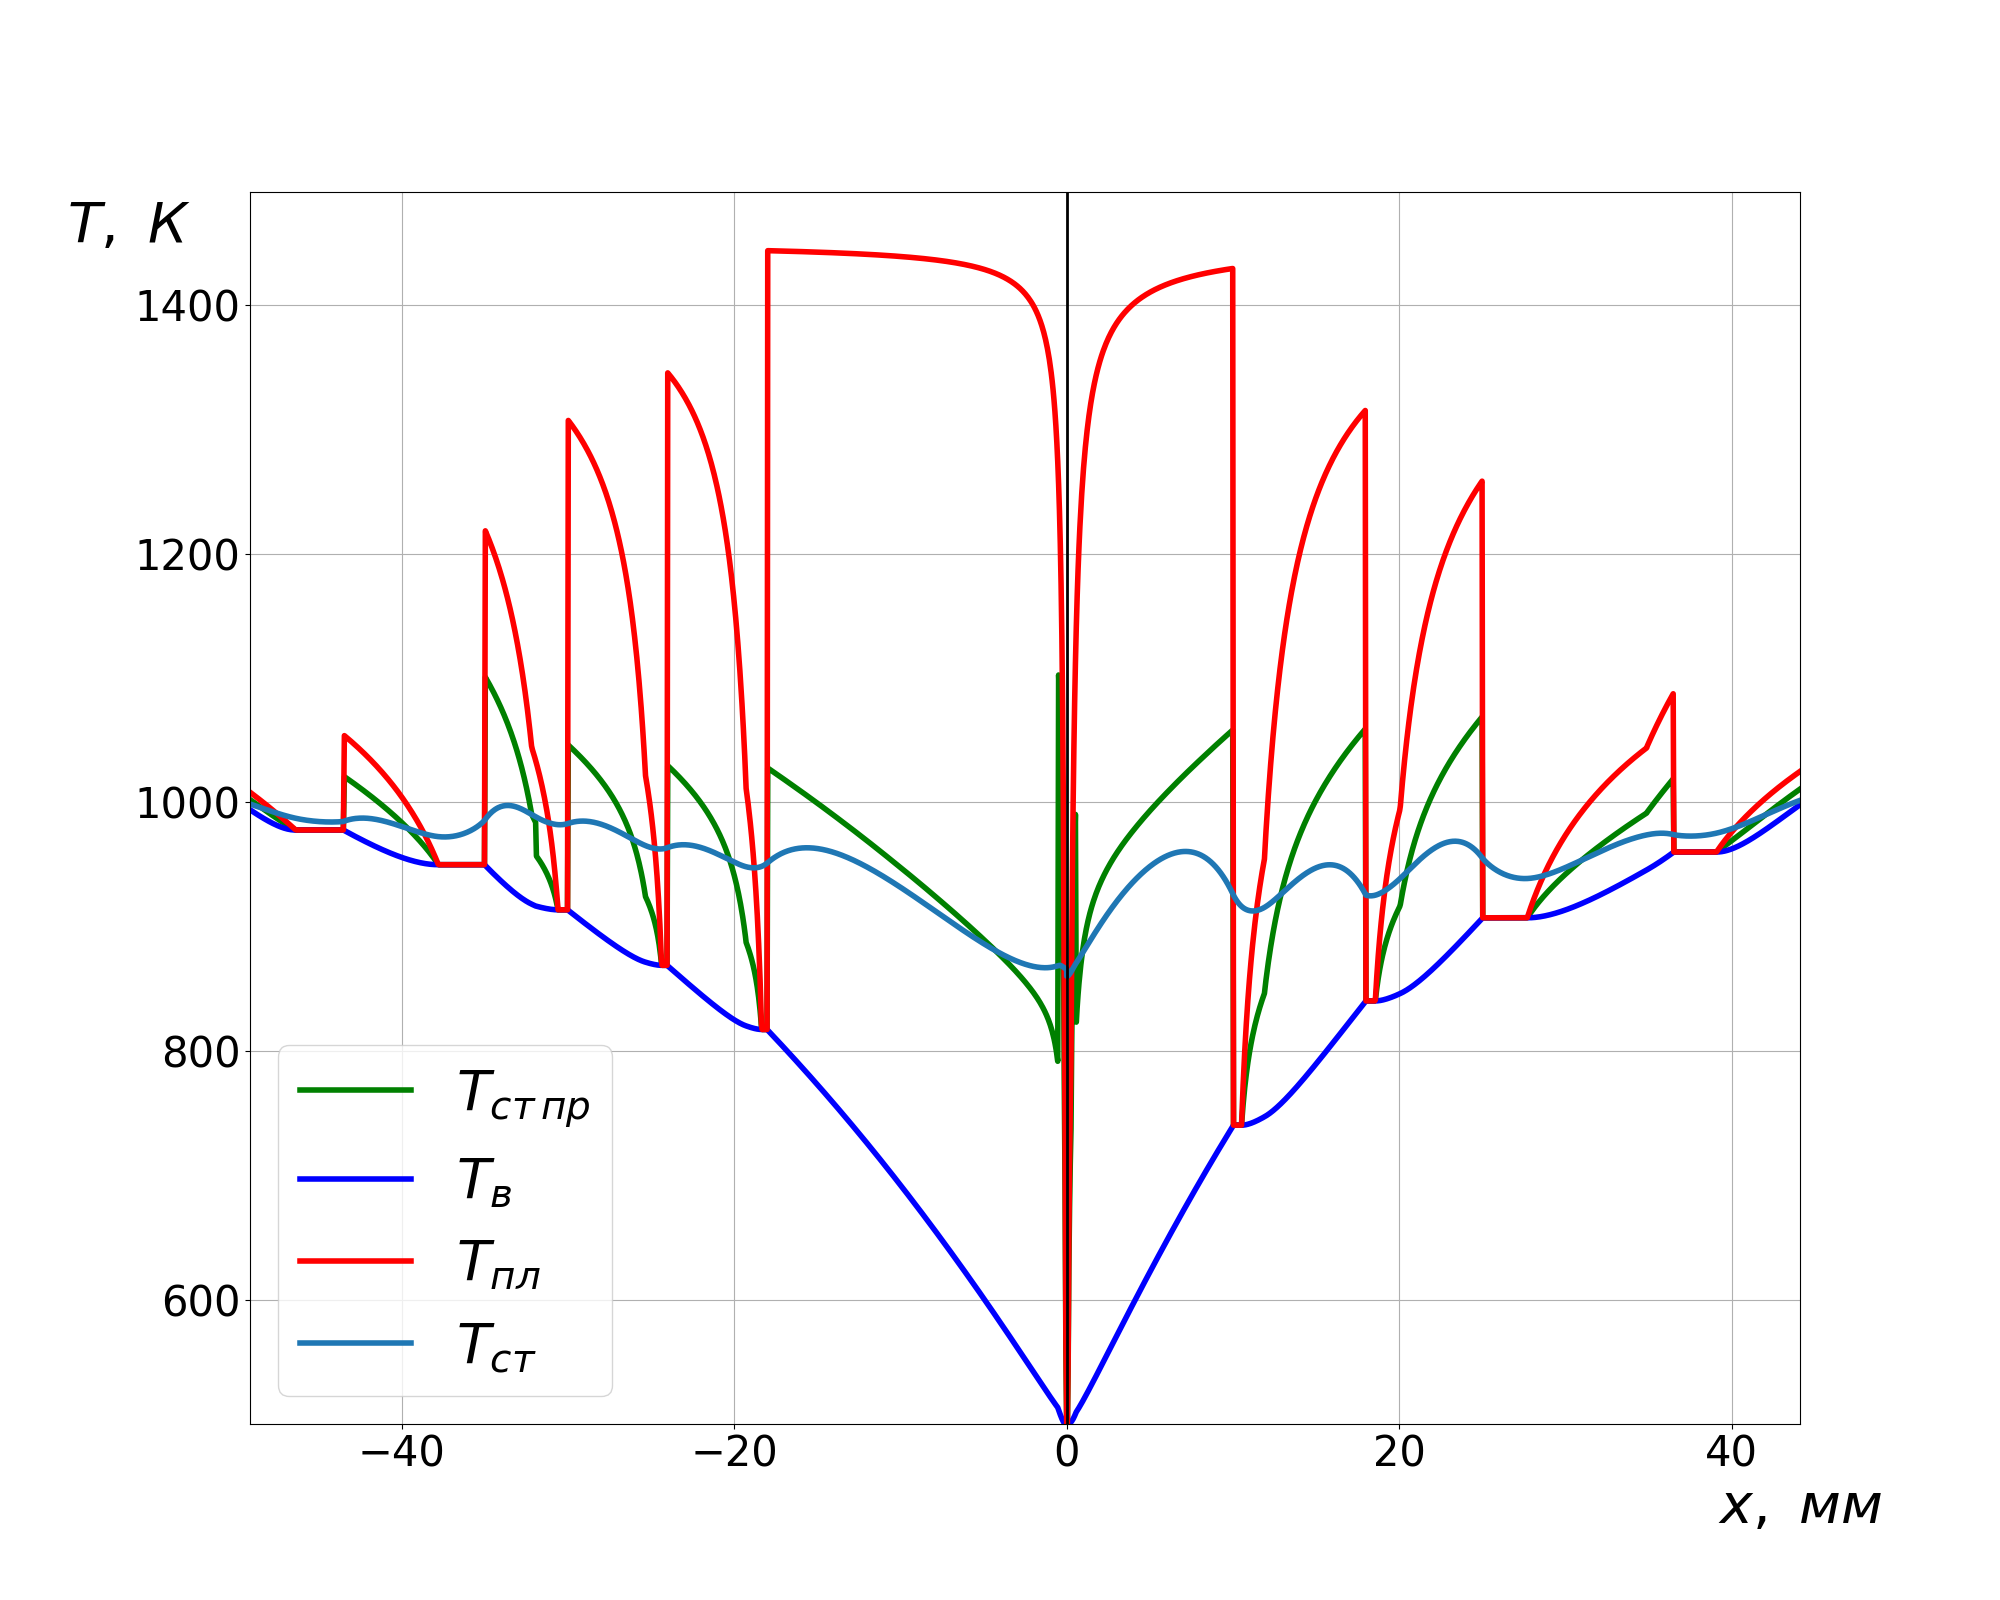
\includegraphics[scale=0.3]{cooling_2_t_front}
	\caption{Распределение температур газа, воздуха и металла (с выдувом в лобовую кромку), $T_{ст \ пр}$ - температура материала лопатки, полученная
	по приближенном методике, $T_в$ - температура охлаждающего воздуха, $T_{пл}$ - температура пленки, $T_{ст}$ -
	температура материала лопатки, полученная по уточненной методике}
	\label{img:cool_gas_parameters_front}
\end{figure}

Таким образом, из расчета следует, что ни в одной точке температура материала лопатки не превышает 1000 К (максимальная температура
равна 998 К), что обеспечивает достаточную прочность лопаток
~\cite{js_36_properties}.

Из сравнения полученных распределений можно заметить, что выдув в лобовой точке приводит к существенному уменьшнию
неравномерности температуры материала сопловой лопатки (с 256,7 до 141,4 К), что приводит к увеличению ресурса горячей
части, так как коррозия и термические напряжения являются основными причинами разрушения сопловых лопаток турбины.